\section{Aprendizaje Estadístico}


%%%%%%%%%%%%%%%%%%%%%%%%%%%%%%%%%%%%%%%%%%%%%%%%%%%%%%%%%%%%%%%%%%%%%%%%%%%%%%%%%%%%
%%%%%%%%%%%%%%%%%%%%%%%%%%%%%%%%%%%%%%%%%%%%%%%%%%%%%%%%%%%%%%%%%%%%%%%%%%%%%%%%%%%%
%%%%%%%%%%%%%%%%%%%%%%%%%%%%%%%%%%%%%%%%%%%%%%%%%%%%%%%%%%%%%%%%%%%%%%%%%%%%%%%%%%%%

\subsection{Introducción}

    \begin{frame}
        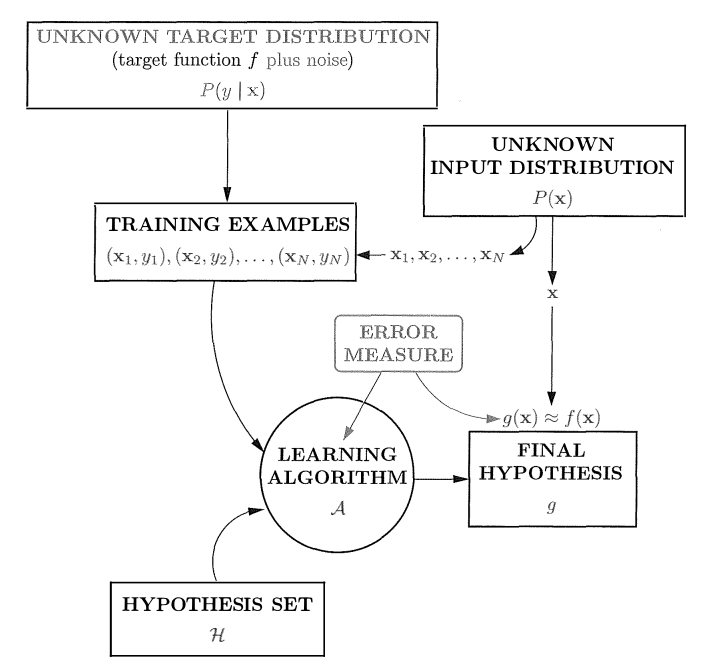
\includegraphics[keepaspectratio=true,height=0.80\paperheight,width=1\paperwidth]{Images/Esquema AASupervisado.png}
    \end{frame}



%%%%%%%%%%%%%%%%%%%%%%%%%%%%%%%%%%%%%%%%%%%%%%%%%%%%%%%%%%%%%%%%%%%%%%%%%%%%%%%%%%%%
%%%%%%%%%%%%%%%%%%%%%%%%%%%%%%%%%%%%%%%%%%%%%%%%%%%%%%%%%%%%%%%%%%%%%%%%%%%%%%%%%%%%
%%%%%%%%%%%%%%%%%%%%%%%%%%%%%%%%%%%%%%%%%%%%%%%%%%%%%%%%%%%%%%%%%%%%%%%%%%%%%%%%%%%%
    
\subsection{ERM}

   \begin{frame}
       \begin{definition}[Error Empírico]
          Dada $h\in \mathcal{H}$ y  ${S=\{(x_1,y_1),...,(x_m,y_m)\}}$ un conjunto de entrenamiento, se define el error empírico como 
                \begin{equation}
                \hat{R}_{S}(h) := \frac{1}{m} \sum_{i=1}^m [\mathbb{I}_{h(x_i) \not= y_i}]
                \end{equation}
       \end{definition}
       
       \pause
       
       \begin{definition}[Error de Generalización - Clasificación Binaria]\label{def:errorGeneralizacion}
            Dada $h \in \mathcal{H}$, una función objetivo $f$ y una distribución de probabilidad $P$ definimos el error de generalización de $h$ como
            \begin{equation}
                R_{P,f}(h) := \mathbb{P}_{x \sim P}[h(x) \neq f(x)] = P(\{x: h(x) \neq f(x)\}) \quad \forall x \in \mathcal{X}
            \end{equation}
        \end{definition}
        
        \pause  
        
        \begin{Criterio}
        Se elige una hipótesis $h_S \in \mathcal{H}$ tal que $h_S \in argmin_{h \in \mathcal{H}}\hat{R}_S(h)$
        \end{Criterio}
        
   \end{frame}
   
   
   
%%%%%%%%%%%%%%%%%%%%%%%%%%%%%%%%%%%%%%%%%%%%%%%%%%%%%%%%%%%%%%%%%%%%%%%%%%%%%%%%%%%%
%%%%%%%%%%%%%%%%%%%%%%%%%%%%%%%%%%%%%%%%%%%%%%%%%%%%%%%%%%%%%%%%%%%%%%%%%%%%%%%%%%%%
%%%%%%%%%%%%%%%%%%%%%%%%%%%%%%%%%%%%%%%%%%%%%%%%%%%%%%%%%%%%%%%%%%%%%%%%%%%%%%%%%%%%

\subsection{Aprendizaje Correcto Probablemente Aproximado}

\begin{frame}
    
    \begin{postulate}[Asunción de realizabilidad]
    Se supone que existe $h^*\in \mathcal{H}$ tal que $R_{P,f}(h^*) = 0$
    \end{postulate}
    
    \pause

    \begin{definition}[Aprendizaje PAC]
        Una clase de hipótesis $\mathcal{H}$ es PAC aprendible cuando exista una función $m_{\mathcal{H}}:(0,1)^2 \to \mathbb{N}$ y un algoritmo de aprendizaje $\mathcal{A}$ con la siguiente propiedad: Para todo $\epsilon, \delta \in (0,1)$, para cada distribución $P$ sobre $\mathcal{X}$ y para cada función objetivo $f:\mathcal{X} \to \{0,1\}$, si se cumple la hipótesis de realizabilidad con respecto $\mathcal{H}, P,f$, entonces cuando ejecutamos el algoritmo de aprendizaje $\mathcal{A}$ en $m \geq m_{\mathcal{H}}(\epsilon,\delta)$ $i.i.d.$ ejemplos generados por $P$ y etiquetados por $f$, $\mathcal{A}$ devuelve una hipótesis $h \in \mathcal{H}$ tal que,
        
            \begin{equation}
                \mathbb{P}_{S\sim P^m}[R_{P,f}(h) \leq \epsilon] \geq 1 - \delta
            \end{equation}
    \end{definition}
    
\end{frame}


\begin{frame}

    \begin{overprint} %En el mismo frame metemos varias diapositivas que se sobreescriben
        
        % Diapo 1
        \onslide<1> 
            \begin{proposition}
            Bajo la asunción de realizabilidad, toda clase de hipótesis finita es PAC aprendible verificando, 
                \begin{equation*}
                    m_{\mathcal{H}} (\epsilon, \delta) \leq \lceil \frac{log(|\mathcal{H}|/\delta)}{\epsilon} \rceil
                \end{equation*}
            \end{proposition}
        % Diapo 2
        \onslide<2>
            \begin{proposition}
            Bajo la asunción de realizabilidad, toda clase de hipótesis finita es PAC aprendible verificando, 
                \begin{equation*}
                    m_{\mathcal{H}} (\epsilon, \delta) \leq \lceil \frac{log(|\mathcal{H}|/\delta)}{\epsilon} \rceil
                \end{equation*}
            \end{proposition}
            pero...
        % Diapo 3
        \onslide<3>
            \begin{proposition}
            Bajo la asunción de realizabilidad, toda clase de hipótesis finita es PAC aprendible verificando, 
                \begin{equation*}
                    m_{\mathcal{H}} (\epsilon, \delta) \leq \lceil \frac{log(|\mathcal{H}|/\delta)}{\epsilon} \rceil
                \end{equation*}
            \end{proposition}
            ¿Qué pasa si eliminamos la asunción de realizabilidad?
        % Diapo 4
        \onslide<4>
            \begin{proposition}
            Bajo la asunción de realizabilidad, toda clase de hipótesis finita es PAC aprendible verificando, 
                \begin{equation*}
                    m_{\mathcal{H}} (\epsilon, \delta) \leq \lceil \frac{log(|\mathcal{H}|/\delta)}{\epsilon} \rceil
                \end{equation*}
            \end{proposition}
            
            ¿Qué pasa si eliminamos la asunción de realizabilidad? \\
            
            ¿Qué pasa cuando la clase de hipótesis es infinita?
        % Diapo 5  
        \onslide<5>
            \begin{proposition}
            Bajo la asunción de realizabilidad, toda clase de hipótesis finita es PAC aprendible verificando, 
                \begin{equation*}
                    m_{\mathcal{H}} (\epsilon, \delta) \leq \lceil \frac{log(|\mathcal{H}|/\delta)}{\epsilon} \rceil
                \end{equation*}
            \end{proposition}
            
            ¿Qué pasa si eliminamos la asunción de realizabilidad? 
            \begin{center} \textbf{Aprendizaje PAC Agnóstico + Convergencia Uniforme} \\ \end{center}
            ¿Qué pasa cuando la clase de hipótesis es infinita? 
            \begin{center} \textbf{Dimensión de Vapnik-Chervonenkis} \end{center}
    \end{overprint}
\end{frame}




\begin{frame}{Aprendizaje PAC Agnóstico}
    \begin{overprint}
    
        \onslide<1>
        Eliminamos la asunción de realizabilidad y definimos...
        
        \onslide<2>
            \begin{definition}[Aprendizaje PAC Agnóstico]
            Una clase de hipótesis $\mathcal{H}$ es PAC Agnóstica con respecto a un conjunto $Z \subset \mathcal{X} \times \mathcal{Y}$ y una función de pérdida medible $\ell: \mathcal{H} \times Z \to \mathbb{R}^+$ cuando exista una función $m_{\mathcal{H}}:(0,1)^2 \to \mathbb{N}$ y un algoritmo de aprendizaje $\mathcal{A}$ cumpliendo la siguiente propiedad: Para cada $\epsilon ,\delta \in (0,1)$ y para cada distribución $P$ sobre $Z$, cuando ejecutamos el algoritmo de aprendizaje sobre  $m \geq m_{\mathcal{H}}(\epsilon, \delta)$ ejemplos $i.i.d.$ generados por $P$, el algoritmo devuelve $h \in \mathcal{H}$ tal que,
            
            \begin{equation}
                \mathbb{P}_{S \sim P}[L_P(h) - min_{h' \in \mathcal{H}} L_P(h') \leq \epsilon] \geq 1 - \delta
            \end{equation}
            
            donde $L_P(h) = \mathbb{E}_{z\sim P}[\ell(h,z)]$ 
            \end{definition}
            
    \end{overprint}
\end{frame}



\begin{frame}{Convergencia Uniforme}
    
    \begin{definition}[Convergencia uniforme]
       Decimos que una clase de hipótesis $\mathcal{H}$ cumple la propiedad de la convergencia uniforme (con respecto a un dominio $Z$ y una función de error $\ell$) cuando exista una función $m_{\mathcal{H}}^{UC}:(0,1)^2 \to \mathbb{N}$ tal que para cada $\epsilon, \delta \in (0,1)$ y para cada distribución de probabilidad, $P$, sobre $Z$, si el conjunto de entrenamiento, $S$, tiene $m \geq m_{\mathcal{H}}^{UC}(\epsilon,\delta)$ ejemplos tomados de manera $(i.i.d.)$ de acuerdo a $P$, entonces con probabilidad al menos $1-\delta$ se cumple,
           \begin{equation}
            |\hat{R}_{S}(h) - R_{P,f}(h)| \leq \epsilon \quad \forall h \in \mathcal{H}
           \end{equation}
    \end{definition}
    
\end{frame}



\begin{frame}{Resultado}
    \begin{proposition}
        Si una clase de hipótesis cumple la propiedad de convergencia uniforme entonces es PAC agnóstica aprendible con una complejidad de la muestra ${m_{H}(\epsilon,\delta) \leq m_{\mathcal{H}}^{UC}(\frac{\epsilon}{2},\delta)}$.
    \end{proposition}
    
\end{frame} 



%%%%%%%%%%%%%%%%%%%%%%%%%%%%%%%%%%%%%%%%%%%%%%%%%%%%%%%%%%%%%%%%%%%%%%%%%%%%%%%%%%%%
%%%%%%%%%%%%%%%%%%%%%%%%%%%%%%%%%%%%%%%%%%%%%%%%%%%%%%%%%%%%%%%%%%%%%%%%%%%%%%%%%%%%
%%%%%%%%%%%%%%%%%%%%%%%%%%%%%%%%%%%%%%%%%%%%%%%%%%%%%%%%%%%%%%%%%%%%%%%%%%%%%%%%%%%%

\subsection{Dimensión Vapnik-Chervonenkis}

\begin{frame}{Definiciones Principales}
    
    \begin{definition}[función de crecimiento]
         Sea $\mathcal{H}$ una clase de hipótesis. La función de crecimiento de $\mathcal{H}$, $m_{\mathcal{H}}:\mathbb{N} \to \mathbb{N}$ se define como 
         \begin{equation}
         m_{\mathcal{H}}(N) = \underset{x_1,...,x_N \in \mathcal{X}}{max} |\mathcal{H}(x_1,...,x_N)|
         \end{equation}
     \end{definition}
     
    \pause
     
    \begin{definition}[Dimensión Vapnik-Chervonenkis]
    La dimensión VC de una clase de hipótesis $\mathcal{H}$ se define como  ${d_{VC}(\mathcal{H}) = \max \{N \in \mathbb{N} : m_{\mathcal{H}}(N) = 2^N\} }$. Si $m_{\mathcal{H}}(N) = 2^N$ para todo $N$, entonces $d_{VC}(\mathcal{H}) = \infty$.
    \end{definition}
    
    \pause
    
    \begin{proposition}
    Sea $\mathcal{H}$ una clase de hipótesis tal que $d_{VC}(\mathcal{H}) = \infty$, entonces $\mathcal{H}$ no es PAC aprendible.
    \end{proposition}
    
\end{frame}     


%%%%%%%%%%%%%%%%%%%%%%%%%%%%%%%%%%%%%%%%%%%%%%%%%%%%%%%%%%%%%%%%%%%%%%%%%%%%%%%%%%%%
%%%%%%%%%%%%%%%%%%%%%%%%%%%%%%%%%%%%%%%%%%%%%%%%%%%%%%%%%%%%%%%%%%%%%%%%%%%%%%%%%%%%
%%%%%%%%%%%%%%%%%%%%%%%%%%%%%%%%%%%%%%%%%%%%%%%%%%%%%%%%%%%%%%%%%%%%%%%%%%%%%%%%%%%%
\subsection{Teorema Fundamental del Aprendizaje Estadístico}

\begin{frame}{Primer resultado más importante}
    
    \begin{theorem}[Teorema Fundamental del aprendizaje estadístico]
        Sea $\mathcal{H}$ una clase de hipótesis que van de $\mathcal{X}$ a $\{0,1\}$ y sea la función de pérdida $\ell = \ell_{0-1}$. Equivalen las siguientes afirmaciones:
        \begin{enumerate}
                \item $\mathcal{H}$ cumple la propiedad de convergencia uniforme
                \item El criterio ERM garantiza que $\mathcal{H}$ sea PAC agnóstica aprendible
                \item $\mathcal{H}$ es PAC agnóstica aprendible
                \item $\mathcal{H}$ es PAC aprendible
                \item El criterio ERM garantiza que $\mathcal{H}$ sea PAC aprendible
                \item $\mathcal{H}$ tiene una dimensión VC finita
            \end{enumerate}
    \end{theorem}
\end{frame}



%%%%%%%%%%%%%%%%%%%%%%%%%%%%%%%%%%%%%%%%%%%%%%%%%%%%%%%%%%%%%%%%%%%%%%%%%%%%%%%%%%%%
%%%%%%%%%%%%%%%%%%%%%%%%%%%%%%%%%%%%%%%%%%%%%%%%%%%%%%%%%%%%%%%%%%%%%%%%%%%%%%%%%%%%
%%%%%%%%%%%%%%%%%%%%%%%%%%%%%%%%%%%%%%%%%%%%%%%%%%%%%%%%%%%%%%%%%%%%%%%%%%%%%%%%%%%%
\subsection{Cotas de Generalización}

\begin{frame}
        Partimos de la desigualdad de Hoeffding:
        \begin{equation*}
            \mathbb{P} \Big[ \Big| \hat{R}_S(g) - R_{P}(g) \Big| \geq \epsilon \Big] \leq 2 e^{-2m\epsilon^2 }
        \end{equation*}
        \pause
        \begin{itemize}
            \item Fijada una hipótesis $g \in \mathcal{H}$: \begin{equation*}
                 R_P(g) \leq \hat{R}_S(g) + \sqrt{\frac{1}{2m}\log{\frac{2}{\delta}}}
             \end{equation*}
        \pause             
             \item $\mathcal{H}$ finito y consistente:          \begin{equation*}
            R_P(h_S) \leq \frac{1}{m}\Big( \log\Big(\frac{|\mathcal{H}|}{\delta}\Big) \Big) 
         \end{equation*}
        \pause
             
             
             \item $\mathcal{H}$ finito y no consistente:             \begin{equation*}
            \forall h \in \mathcal{H}, \quad R(h) \leq \hat{R}(h) + \sqrt{\frac{1}{2m} \log \Big( \frac{2|\mathcal{H}|}{\delta} \Big)}
            \end{equation*}
        \end{itemize}
\end{frame}



\begin{frame}{Segundo resultado más importante}
    \begin{theorem}[Cota de generalización VC]
        Para cualquier tolerancia $\delta \in (0,1)$, con probabilidad al menos $1-\delta$ ocurre,
            \begin{equation}
                R(h) \leq \hat{R}(h) + \sqrt{\frac{8}{N}\log\Big(\frac{4m_{\mathcal{H}}(2N)}{\delta}\Big)} \quad \forall h \in \mathcal{H}
            \end{equation}
    \end{theorem}
    
    \pause
    
    \begin{itemize}
        \item Resultado universal.
        \item La cota no es fina.
        \item Establece la viabilidad del aprendizaje con $\mathcal{H}$ infinitos.
        \item Útil para comparar el rendimiento de generalización de distintos modelos.
    \end{itemize}
\end{frame}